\documentclass[a6paper,landscape,10pt]{report}

\usepackage[utf8]{inputenc}
%\usepackage{xltxtra}
\usepackage[portuguese]{babel}
\usepackage[top=1cm,left=.4cm,right=.4cm,bottom=.8cm,footskip=-1cm]{geometry} %Define margens e distância do rodapé
\usepackage{titletoc} %Para definir o estilo da lista de conteúdo
\usepackage[toc]{multitoc} %Para lista de conteúdo com 3 colunas
\usepackage{pdfpages} %Para incluir pdfs
\usepackage{fancyhdr} %Para personalizar cabeçalho e rodapé
\usepackage[none]{hyphenat} %Impedir quebra de palavras no fim da linha
\usepackage[pdftex]{hyperref}
\usepackage{xcolor}
\usepackage{afterpage}

\hypersetup{
    colorlinks,
    citecolor=black,
    filecolor=black,
    linkcolor=black,
    urlcolor=black
    pdfauthor={Gabriel Fonseca},
    pdfsubject={carnaval},
    pdftitle={Songbook do Carnaval},
    pdfcreator={Gabriel Fonseca},
    pdfproducer={Gabriel Fonseca}
}
%Fonte padrão Sans Serif, na verdade só pro índice...
\usepackage{PTSansNarrow}
\renewcommand*\familydefault{\sfdefault}
\usepackage[T1]{fontenc}
%\usepackage{Intro}

%Define novo estilo de cabeçalho e rodapé
\fancypagestyle{plain}{%
  \renewcommand{\headrulewidth}{0pt}%Sem linha de cabeçalho
  \fancyfoot[C]{} %Sem nada no centro do rodapé
  \fancyfoot[R]{\fontfamily{phv}\selectfont\Large\textbf{\thepage}} %Número da página grande e em negrito à direita do rodapé
}

\renewcommand*{\multicolumntoc}{3} %Define 3 colunas para a lista de conteúdo

\newcommand{\musica}[1]{\phantomsection\addcontentsline{toc}{section}{#1}}
\newcommand{\capitulo}[1]{\phantomsection\addcontentsline{toc}{chapter}{#1}}

%Define estilo dos capítulos no índice
\titlecontents{chapter}
[.3cm] %espaço à esquerda
{\addvspace{.8em}\bf\contentsmargin{0em}} %formatação do título e espaço vertical antes
{} %formato de número
{} %formato de número sem título
{\vspace*{.4em}} %filler
[] %espaço depois do título

%Define estilo da seção no índice
\titlecontents{section}
[.2cm] %espaço à esquerda
{\small} %formatação do título e espaço vertical antes
{} %formato de número
{\textbf{\contentspage}\hspace{2em}} %formato de número sem título
{\hfill} %filler
[] %espaço depois do título


\newcommand{\tom}{BB}

\begin{document}

%Sem numeração nas primeiras páginas
\pagestyle{empty}

%\capa{capa}
\newgeometry{top=1cm,left=.4cm,right=.4cm,bottom=.2cm,footskip=0cm}
\pagecolor{black}\afterpage{\nopagecolor\restoregeometry}
{\color{white} \bf

\usefont{T1}{Intro-TLF}{m}{n}

\vspace*{\fill}

\noindent
\resizebox{.2\textwidth}{!}{2016 . BB}

\begin{center}
  \rule{\textwidth}{5 pt}

  \bigskip
  \resizebox{\textwidth}{!}{SOPRA QUE}

  \bigskip
  \resizebox{\textwidth}{!}{\usefont{T1}{IntroInline-TLF}{m}{n} SARA!}

  \bigskip
  \rule{\textwidth}{5 pt}
\end{center}
}
\newpage


%Cria lista de conteúdo sem cabeçalho
% \begingroup
% \makeatletter
% \@starttoc{toc}
% \makeatother
% \endgroup

%Define estilo das páginas incluídas como PDF
\includepdfset{pagecommand={\thispagestyle{plain}}}

%Começa o livro
\newpage
\musica{Bandeira Branca}
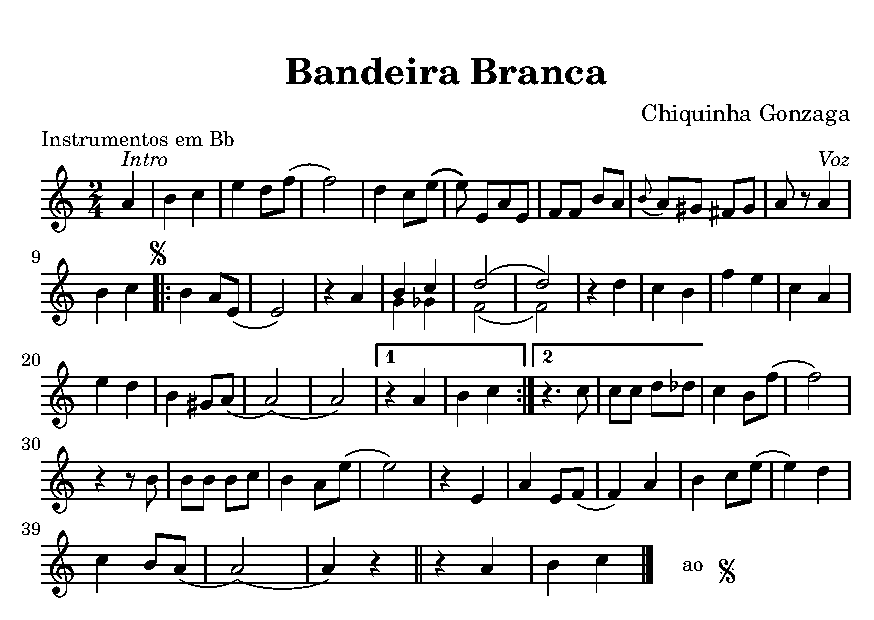
\includepdf{../PDF/bandeiraBranca.pdf}

\musica{As Pastorinhas}
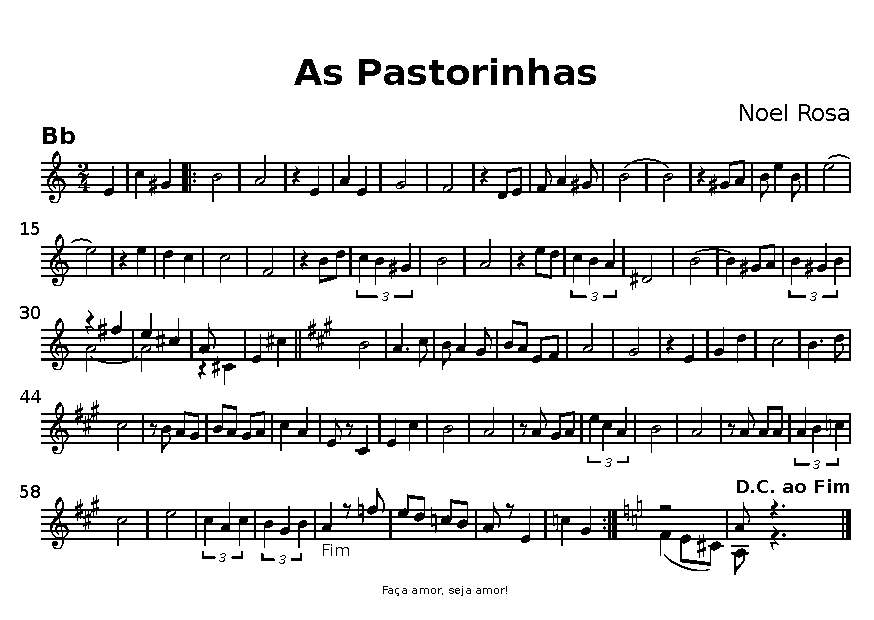
\includepdf{../PDF/pastorinhas.pdf} %Inclui a partitura no songbook

\musica{Máscara Negra}
\includepdf{../PDF/mascara.pdf}

\musica{Ô Abre Alas}
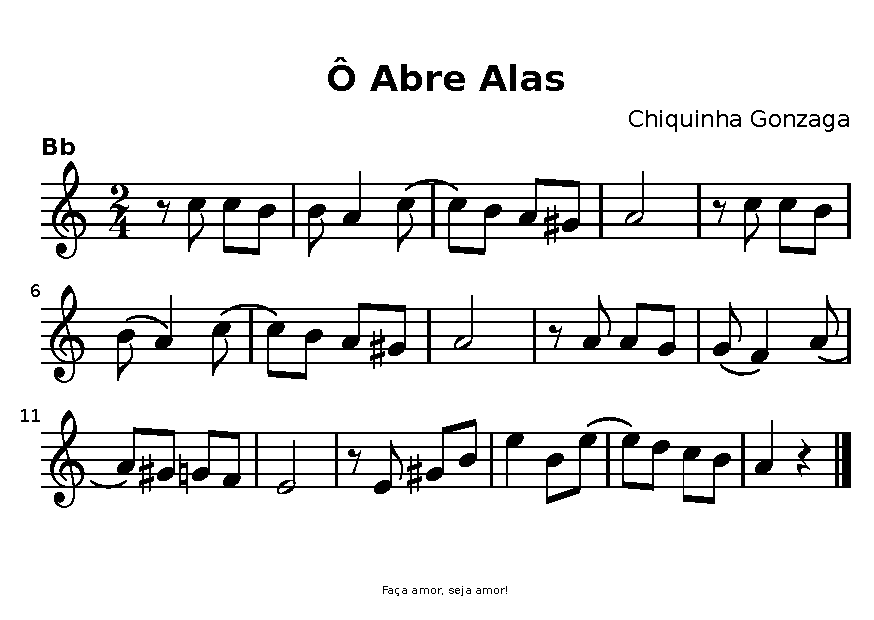
\includepdf{../PDF/abreAlas.pdf}

\musica{Aurora}
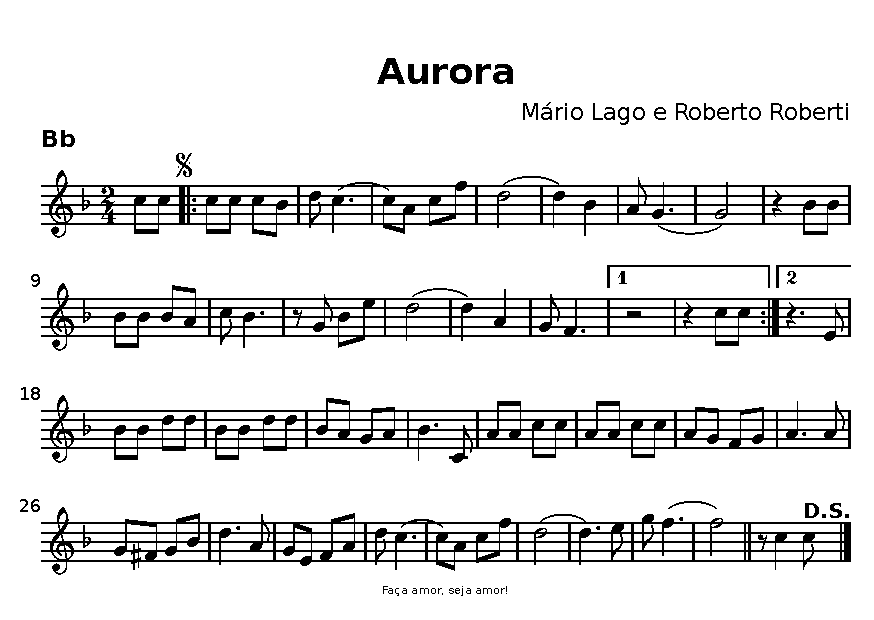
\includepdf{../PDF/aurora.pdf}

\musica{Cabeleira do Zezé}
\includepdf{../PDF/cabeleiraDoZeze.pdf}

\musica{Cachaça}
\includepdf{../PDF/cachaca.pdf}

\musica{Coração de Jacaré}
\includepdf{../PDF/coracaoDeJacare.pdf}

\musica{Índio quer apito}
\includepdf{../PDF/indio.pdf}

\musica{A Jardineira}
\includepdf{../PDF/jardineira.pdf}

\musica{Mamãe eu Quero}
\includepdf{../PDF/mamaeEuQuero.pdf}

\musica{Marcha da Cueca}
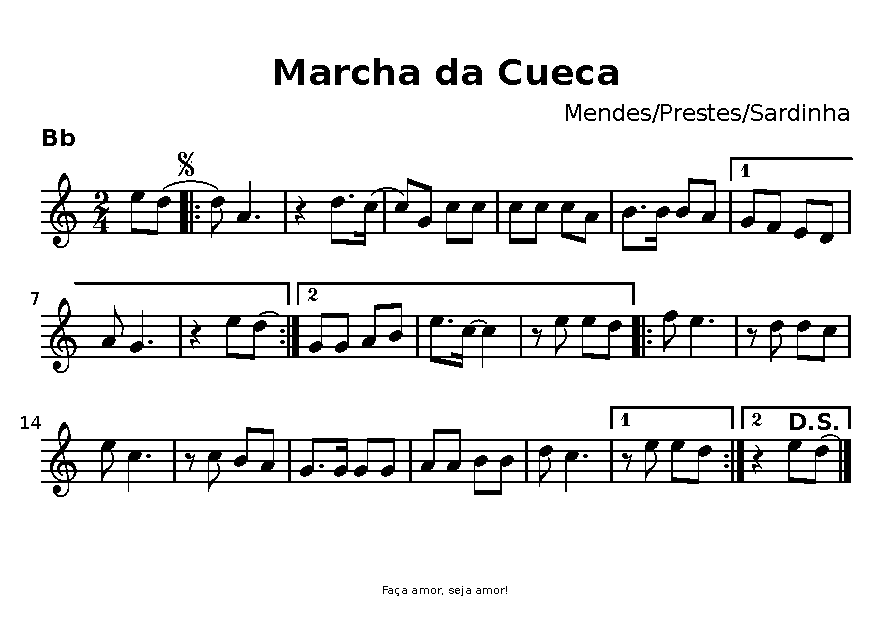
\includepdf{../PDF/marchaDaCueca.pdf}

\musica{Marcha do Remador}
\includepdf{../PDF/remador.pdf}

\musica{Maria Sapatão}
\includepdf{../PDF/mariaSapatao.pdf}

\end{document}
